% --------------------------------------------------------------------------- %
% Poster for the ECCS 2011 Conference about Elementary Dynamic Networks.      %
% --------------------------------------------------------------------------- %
% Created with Brian Amberg's LaTeX Poster Template. Please refer for the     %
% attached README.md file for the details how to compile with `pdflatex`.     %
% --------------------------------------------------------------------------- %
% $LastChangedDate:: 2011-09-11 10:57:12 +0200 (V, 11 szept. 2011)          $ %
% $LastChangedRevision:: 128                                                $ %
% $LastChangedBy:: rlegendi                                                 $ %
% $Id:: poster.tex 128 2011-09-11 08:57:12Z rlegendi                        $ %
% --------------------------------------------------------------------------- %
\documentclass[a0paper,portrait]{baposter}

\usepackage{relsize}		% For \smaller
\usepackage{url}			% For \url
\usepackage{epstopdf}	% Included EPS files automatically converted to PDF to include with pdflatex
\usepackage[utf8x]{inputenc}
\usepackage{mathptmx}
\usepackage{amsmath}


%%% Global Settings %%%%%%%%%%%%%%%%%%%%%%%%%%%%%%%%%%%%%%%%%%%%%%%%%%%%%%%%%%%

\graphicspath{{pix/}}	% Root directory of the pictures 
\tracingstats=2			% Enabled LaTeX logging with conditionals

%%% Color Definitions %%%%%%%%%%%%%%%%%%%%%%%%%%%%%%%%%%%%%%%%%%%%%%%%%%%%%%%%%

\definecolor{bordercol}{RGB}{160,160,160}
\definecolor{headercol1}{RGB}{255,255,255}
\definecolor{headercol2}{RGB}{160,160,160}
\definecolor{headerfontcol}{RGB}{0,0,0}
\definecolor{boxcolor}{RGB}{255,255,255}

%%%%%%%%%%%%%%%%%%%%%%%%%%%%%%%%%%%%%%%%%%%%%%%%%%%%%%%%%%%%%%%%%%%%%%%%%%%%%%%%
%%% Utility functions %%%%%%%%%%%%%%%%%%%%%%%%%%%%%%%%%%%%%%%%%%%%%%%%%%%%%%%%%%

%%% Save space in lists. Use this after the opening of the list %%%%%%%%%%%%%%%%
\newcommand{\compresslist}{
	\setlength{\itemsep}{1pt}
	\setlength{\parskip}{0pt}
	\setlength{\parsep}{0pt}
}

%%%%%%%%%%%%%%%%%%%%%%%%%%%%%%%%%%%%%%%%%%%%%%%%%%%%%%%%%%%%%%%%%%%%%%%%%%%%%%%
%%% Document Start %%%%%%%%%%%%%%%%%%%%%%%%%%%%%%%%%%%%%%%%%%%%%%%%%%%%%%%%%%%%
%%%%%%%%%%%%%%%%%%%%%%%%%%%%%%%%%%%%%%%%%%%%%%%%%%%%%%%%%%%%%%%%%%%%%%%%%%%%%%%

\begin{document}
\typeout{Poster rendering started}

%%% Setting Background Image %%%%%%%%%%%%%%%%%%%%%%%%%%%%%%%%%%%%%%%%%%%%%%%%%%
\background{
	\begin{tikzpicture}[remember picture,overlay]%
	\draw (current page.north west)+(-2em,2em) node[anchor=north west]
	{
\includegraphics[height=1.2\textheight]{bl}};
	\end{tikzpicture}
}

%%% General Poster Settings %%%%%%%%%%%%%%%%%%%%%%%%%%%%%%%%%%%%%%%%%%%%%%%%%%%
%%%%%% Eye Catcher, Title, Authors and University Images %%%%%%%%%%%%%%%%%%%%%%
\begin{poster}{
	grid=false,
	% Option is left on true though the eyecatcher is not used. The reason is
	% that we have a bit nicer looking title and author formatting in the headercol
	% this way
	%eyecatcher=false, 
	borderColor=bordercol,
	headerColorOne=headercol1,
	headerColorTwo=headercol2,
	headerFontColor=headerfontcol,
	% Only simple background color used, no shading, so boxColorTwo isn't necessary
	boxColorOne=boxcolor,
	headershape=roundedright,
	headerfont=\Large\sf\bf,
	textborder=rectangle,
	background=user,
	headerborder=open,
  boxshade=plain
}
%%% Eye Cacther %%%%%%%%%%%%%%%%%%%%%%%%%%%%%%%%%%%%%%%%%%%%%%%%%%%%%%%%%%%%%%%
{
	Eye Catcher, empty if option eyecatcher=false - unused
}
%%% Title %%%%%%%%%%%%%%%%%%%%%%%%%%%%%%%%%%%%%%%%%%%%%%%%%%%%%%%%%%%%%%%%%%%%%
{\sf\bf
	¿Qué se mueve realmente?
}
%%% Authors %%%%%%%%%%%%%%%%%%%%%%%%%%%%%%%%%%%%%%%%%%%%%%%%%%%%%%%%%%%%%%%%%%%
{
	\vspace{1em} Carlos Alí Medina Leal\\
	{\smaller  Licenciatura en física, diciembre de 2014, Cali.medina5423@gmail.com}
}
%%% Logo %%%%%%%%%%%%%%%%%%%%%%%%%%%%%%%%%%%%%%%%%%%%%%%%%%%%%%%%%%%%%%%%%%%%%%
{
% The logos are compressed a bit into a simple box to make them smaller on the result
% (Wasn't able to find any bigger of them.)
\setlength\fboxsep{0pt}
\setlength\fboxrule{0pt}
	\fbox{
		\begin{minipage}{10em}
			
\includegraphics[width=10em,height=10em]{uni.png}
			%
\includegraphics[width=4em,height=4em]{elte_logo} \\
			%
\includegraphics[width=10em,height=4em]{dynanets_logo}
			%
\includegraphics[width=4em,height=4em]{aitia_logo}
		
		\end{minipage}
	}
}

\headerbox{Resumen}{name=problem,column=0,row=0}
{
El movimiento es un fenómeno que vemos día a día a lo largo de nuestra vida, movernos es una acción cotidiana fácil de realizar, pero  ¿Cómo sabemos si no es lo demás lo que se mueve?

En este póster hablaremos sobre el movimiento desde distintos sistemas de referencia, cabe mencionar que este poster fue realizado en base a el libro "$Relatividad$ $para$ $Principiantes$", del autor Shahen Hacyan.

\vspace{0.4em} 	


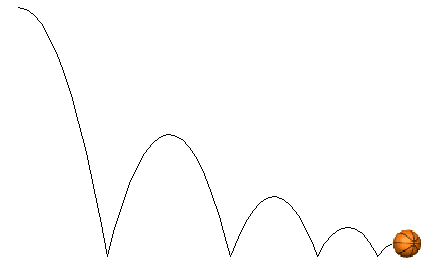
\includegraphics[width=\linewidth,height=12.45em]{pel.png}
}

%\headerbox{Caos determinista}{name=definitions,column=0,below=problem}{
%Uno de los fenómenos más interesantes observados en sistemás dinámicos es el de caos, que está relacionado con 
%la imposibilidad práctica de predecir la evolución futura del sistema

%}

\headerbox{Conclusión}{name=models,column=2,below=problem}{


Podemos decir que nuestra percepción del movimiento puede ser “confundida” ya que todo depende del sistema de referencia que tomamos. Un ejemplo  claro que pasa en la vida cotidiana y puede que no nos percatemos de ello es la Tierra, que parece que está estable e inmóvil, pero en realidad gira al rededor del Sol bastante rápido.  

\begin{center}
	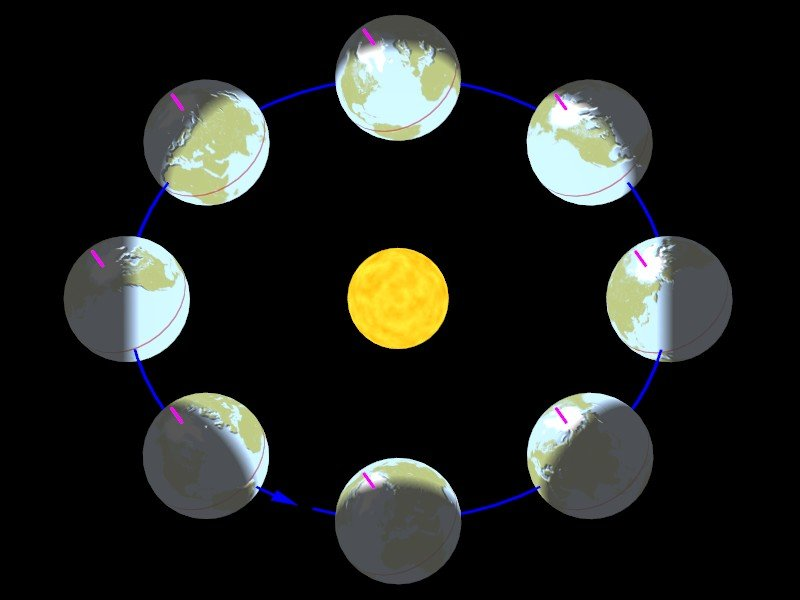
\includegraphics[width=.9\linewidth]{tr.jpg}
	\vspace{0.4em} 
	

\end{center}

Si nuestro sistema de referencia es un barco: el barco está inmóvil. Si nuestro sistema es la Tierra; el barco se mueve y la Tierra es estable. Si nuestro sistema es el Sistema Solar; la Tierra se mueve y el Sistema Solar no. Si tomamos la galaxia; el Sistema Solar se mueve. Etc...
A estas alturas podemos preguntarnos: ¿La piedra en realidad se mueve?

\vspace{0.5em} 

El movimiento está sujetado a los sistemas de referencia que elegimos, y como lo mencionó Galileo, las leyes de la física son independientes de cualquier sistema de referencia, así que hay que reflexionar la próxima vez que digamos que un objeto se mueve. 

}
\headerbox{Referencias}{name=references,span=1,column=2,below=models}{
Shahen Hacyan, $Relatividad$ $para$ $principiantes$, México (2002), Colección La Ciencia para Todos. Texto en base al capítulo I: La Relatividad de Galileo, Pág. 11-17, "Todos los sistemas de referencia son válidos". 
}



\headerbox{Introducción}{name=density,span=2,column=1,row=0}{
La Tierra gira al rededor del Sol a 30 kilómetros por segundo, y éste a su vez a 30 000 kilómetros por segundo alrededor de la vía láctea, que sólo es una galaxia entre millones de galaxias que se alejan unas a otras. Y, sin embargo, no percibimos ninguno de estos movimientos. De hecho, la Tierra parece ser lo único firme e inmutable a nuestro alrededor, y que nos permite realizar mediciones bien definidas que se pueden repetir las veces que queramos, debido a que la Tierra es un excelente $Sistema$ $de$ $referencia$.

	El hecho de que el movimiento de la Tierra sea prácticamente inpercibible en la experiencia cotidiana se debe a un principio que Galileo Galilei enunció claramente en el siglo XVII: Las leyes de la física son independientes de cualquier sistema de referencia.

\begin{center}
	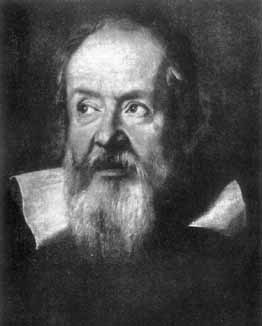
\includegraphics[width=0.23\linewidth]{ga.jpg}
	\vspace{0.4em} 
	
	Galileo Galilei (1564-1642)
\end{center}


}

\headerbox{Sistemas de referencia}
{name=degreeDistribution,span=2,column=0,below=density,above=bottom}
{
En base a un sistema de referencias se pueden estudiar varios fenómenos, sean de la vida diaria o no. Un ejemplo puede ser el movimiento de una piedra que se deja caer de lo alto de un poste: La experiencia nos dice que la piedra caerá exactamente a lo largo de una línea recta vertical (si no soplan vientos fuertes que la desvíen) o con una trayectoria curvada si se empuja horizontalmente.
\vspace{-0.2em}
\begin{center}
	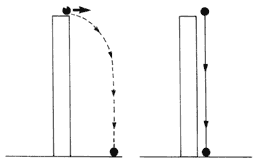
\includegraphics[width=0.41\linewidth]{j.png}

\end{center}

Pero la Tierra no es el único sistema de referencia disponible. ¿Qué pasa si se repite el experimento, pero en un medio en movimiento?
Supongamos que se realiza el experimento en un barco en movimiento, y la piedra se suelta desde lo alto de un mástil. La piedra caería justo al pie del mástil si no fuera por el aire que la empuja hacia atrás. 

Para evitar complicaciones, se puede realizar el experimento en el interior del barco, donde el aire está en reposo. En este caso, la caída de la piedra ocurre exactamente como si el barco no se moviera. 
Pero en cambio, si otro espectador mira el experimento, pero en tierra firme, vería que la trayectoria de la piedra es una parábola .

\begin{center}
	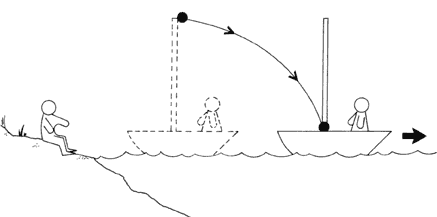
\includegraphics[width=0.7\linewidth]{bah.png}
\end{center}

 Estas dos descripciones de un mismo fenómeno físico son perfectamente compatibles entre sí: un observador en tierra firme ve una piedra que se arroja con una velocidad horizontal que es precisamente la velocidad del barco y ve la piedra caer siempre pegada al mástil, que se mueve con la misma velocidad. Tanto el barco como la tierra firme son sistemas de referencia aceptables, y es sólo
una cuestión de conveniencia escoger el más apropiado.
}


\end{poster}
\end{document}
